\documentclass[a4paper, twocolumn, 11pt]{article}
\usepackage[utf8]{inputenc}
\usepackage[english]{babel}
\usepackage{geometry}
\usepackage{multirow}
\usepackage{longtable}
\usepackage[usenames,dvipsnames]{xcolor}
\bibliographystyle{apalike}
\usepackage{apalike}
\usepackage{mathtools}
\usepackage{graphicx}
\usepackage{amsmath}

\author{Ángela Miranda Segura}
\title{Chlorophyll: its structure, absorption and importance in plants}
\begin{document}
	
\twocolumn[
	\begin{@twocolumnfalse}
	\maketitle
	\begin{center}\rule{0.9\textwidth}{0.1mm} \end{center}
		\begin{abstract}
			https://github.com/angelams98/Proyecto-final\\
			Chlorophyll is any of several related green pigments found in the mesosomes of cyanobacteria and in the chloroplasts of algae and plants. Chlorophyll is essential in photosynthesis, allowing plants to absorb energy from light. This paper deals with the estimation of chlorophyly in plant extracts by application of absorption coefficients of the isolated solid chlorophyll components. 
		\end{abstract}
		\textbf{Keywords:}
		Chlorophyll, function, photosynthesis, plants.
	\begin{center}\rule{0.9\textwidth}{0.1mm} \end{center}
	\end{@twocolumnfalse}
]

\section{Introduction}
 	A leaf with 7 millon cells houses, each containin approximately 600 millon molecules of chlorophyll. These $10^18$ chlorophyll mole-cules, all of which are bound to proteins of photosynthetic membranes, harvest the sunlight. Approximately 250 to 300 of them transfer the absorbed light energy through neighbouting pigments to the "especial pair" chlorophylls in a reaction center. These special pair chlorophylls in photosystems I and II are the primary electron donors that drive the conversion of light into chemical energy to be conserved in NADPH2 and ATP \cite{VonWettstein1995}
 	

	Chlorophylls are esential molecules that are responsible for harvesting solar energy in photosynthetic antenna systemas, and for charge separation and electron transport within reaction centers. Chlorophyll metabolism is a highly coordinated process that is executed via a series of cooperative reactions catalyzed by numerous enzymes.
	
	\subsection{The chlorophyll metabolic\\ pathway and its regulation} 
	Chlorophyll biosynthesis can be classified into three distinct phases (\ref{fig1}). The first phase encompasses the synthesis of chlo-rophyll a from glutamate. Figure 1 depicts the chlorophyll a biosynthetic pathway such that the order of enzymatic steps involving divinyl protochlorophyllide a, \\vinyl reductase, and protochlorophyllide oxidoreductase differs from that in previously proposed schematics describing this pathway. We made this revision on the basis of recent findings describing the substrate specificity of divinyl protochlorophyllide a vinyl reductase. The second phase includes the interconversion of chlorophyll a and chlo-rophyll b, and is also known as the chlorophyll cycle \cite{Rudiger2002}. In this cycle, the in vivo substrate of chlorophyllide a oxygenase (CAO) remains unidentified, although in vitro experiments have shown that chlorophyllide a, rather than chlorophyll a, is a substrate of CAO \cite{Oster2000}. The third and final phase of chlorophyll metabolism involves the degradation of chlorophyll a \cite{Takamiya2000}. This degradation pathway has been traced from chlorophyll a through to the non-fluorescent chlorophyll catabolite (NCC). Clarification is still necessary, however, to determine whether NCC is further degraded to monopyrroles or other smaller molecules. A further question remains as to whether degraded chlorophyll is recycled as a nitrogen resource for building other macromolecules. Although most of the genes that encode the enzymes involved in chlorophyll metabolism have been identified, those encoding some key enzymes such as Mg-dechelatase are still to be identified \cite{Tanaka2006}
	
	\subsection{Catabolic Enzymes and Catabolic Pathway}
	Chlase is a hydrophobic protein of plastid membranes (e.g. 14,32,51,157,172) that is distinguished by its functional latency: In preparations of chloro-plastmembranesChlisnotdephytylatedunlessthemembranesaresolublizedinthe presence of detergent (e.g. 2,93) or acetone at high concentrations (e.g. 32).Even during Chl breakdown in senescent leaves Chlase remains latent. Hence,all the properties of Chlase determined under highly unphysiological condi-tions in vitro, suchas kinetic parameters, dependencies on pH and temperature,and so forth (e.g. 29,66, 81,100,144,173) are likely irrelevant for the under-standing of dephytylation in vivo. The most intriguing problem of regulationof Chl breakdown at the level of Chlase concerns the mechanism by whichthe interaction between Chlase and its substrates is achieved. Latency of theenzyme may be explained simply by the spatial separation between Chl in thethylakoid pigment-protein complexes and Chlase, which appears to be locatedin the plastid envelope (93).\\
	
	P1: PSA/ary P2: NBL/vks QC: KKK/agr T1: KKKMarch 29, 1999 13:51 Annual Reviews AR082-0476 MATILE, H¨ORTENSTEINER \& THOMASChlase is a hydrophobic protein of plastid membranes (e.g. 14,32,51,157,172) that is distinguished by its functional latency: In preparations of chloro-plastmembranesChlisnotdephytylatedunlessthemembranesaresolublizedinthe presence of detergent (e.g. 2,93) or acetone at high concentrations (e.g. 32).Even during Chl breakdown in senescent leaves Chlase remains latent. Hence,all the properties of Chlase determined under highly unphysiological condi-tions in vitro, suchas kinetic parameters, dependencies on pH and temperature,and so forth (e.g. 29,66, 81,100,144,173) are likely irrelevant for the under-standing of dephytylation in vivo. The most intriguing problem of regulationof Chl breakdown at the level of Chlase concerns the mechanism by whichthe interaction between Chlase and its substrates is achieved. Latency of theenzyme may be explained simply by the spatial separation between Chl in thethylakoid pigment-protein complexes and Chlase, which appears to be locatedin the plastid envelope (93).Chlases have been purified repeatedly but despite the availability ofN-terminal amino acid sequences (172,173) and a specific antibody (172), thecorresponding gene(s) has so far been recalcitrant to molecular cloning. Suchunexpected difficulty is not easily explained1. Still another puzzling featureof Chlase is its apparent glycoprotein nature as inferred from binding to con-canavalin A (158,173), indeed an unusual property of a component of chloro-plast envelope membranes.Under certain conditions Chlase can act as a transesterase and, therefore, ithasoccasionally been considered tohavea functionin the phytylation ofChlide(e.g. 30). After the elucidation of the last step of Chl biosynthesis (134), sucha function of Chlase can now be disregarded.\\
	
	PHEOPHORBIDE a OXYGENASE, RCC REDUCTASE The ring-opening step of thecatabolic pathway is decisive for the loss of green color. The first identifiablecolorless product, pFCC (Figure 1) is formally derived from Pheide a by theaddition of two atoms of O and four atoms of H. The enzymic conversion ofPheide a into pFCC in vitro requirestwo protein components from gerontoplastmembranes and stroma, respectively(36, 53,137). Oxygenolysis of Pheide a iscatalyzed by the membrane component, Pheide a oxygenase (PaO), and yieldsthe red bilin RCC that in a channeled reaction is reduced by RCC reductaseto yield pFCC (128) (Figures 1, 2). Chl breakdown in C. protothecoides isterminated by the action of the oxygenase and RCC is released into the culturemedium (26).In Chlorella (20) as well as in Brassica napus (54), incorporation studiesin the presence of18,18O2showed that only the formyl oxygen originates fromdioxygen, whereas the lactam oxygen at C4 is probably derived from water.The mechanismof the monooxygenase-catalyzed ring opening has notyet beenelucidated in detail. A hypothesis has been proposed in which the initial stepis regioselective C4/C5 epoxide formation, followed by hydrolysis and rear-rangement of double bonds (20). Stereoselective final reduction of the C9/C10double bond has been demonstrated (19).Inhibition by appropriate chelators (35) as well as regeneration studies (53)suggest that PaO is an Fe-containing monooxygenase. Its redox cycle is drivenby reduced ferredoxin (Figure 2); in the light, this reductant is generated byphotosystem I (128), whereas in the dark, NADPH and a corresponding sys-tem involving the stromal oxidative pentose-phosphate-cycle and glucose-6-phosphate as ultimate e−donor are required (36,53,128). In senescent leaves,all components of such a reducing system (177), including ferredoxin (128),are retained or even newly synthesized as long as Chl breakdown continues.AmongthepropertiesofPaO,theabsolutespecificityforPheideaassubstrate(53)is noteworthy becauseit explainstheexclusiveoccurrence ofChl a-derivedfinal catabolites (\ref{fig2}). Pheide b is a competitive inhibitor of PaO but is nomore effective as a substrate than pyroPheide, protoporphyrin IX, and Chlidea (S H¨ortensteiner, unpublished data). The oxygenase of C. protothecoidesseems to be less specific, as suggested by the production of an RCC derived from Pheide b (60).So far,theactivityofPaOhasbeendetectedonlyinsenescentleavesofseveralspecies(36,53, 137,167,178)as wellasin ripeningfruits(1, 103). Indeed, PaO appears to be the only enzyme that plays a pace-making role in the breakdownof Chl, and the catabolic pathway (\ref{fig3}) may, therefore, be designated asthe “pheophorbide a pathway.”\\


\section{State of art}
	Results of recent studies have better defined the chlorophyll metabolic pathway,\\ specifically by identifying the majority of the genes that are involved in the process. These recent advances have enabled significant progress toward understanding the me-chanisms that regulate chlorophyll meta-bolism. Regulation of the levels of chlorophyll and its derivatives is extremely important because these molecules are strong photosensitizers; that is, when present in excess, they will generate reactive oxygen species (ROS). ROS, in turn, promote\\ growth retardation or cell death. Therefore, to maintain healthy growth, plants must finely control the entire chlorophyll metabolic process.\\
	
	Additional studies have revealed preliminary information about the mechanisms that govern the trafficking of chlorophyll metabolic intermediates in plants. This level of control is especially important because, in response to cellular demand, plants produce various tetrapyrrole molecules, such as heme, siroheme and phytochromobilin, that are employed further in a variety of biochemical processes. Significant progress has also been made toward elucidating the linkages between chlorophyll metabolism and other cellular processes, including leaf senescence, programmed cell death, and plastid signaling. Although the molecular mechanisms that underlie these linkages remain elusive, these initial findings have motivated us to re-examine the physiological implications of chlorophyll metabolism \cite{Tanaka2006}

\section{Materials and methods}
	It has been studied the absorption of light by chlorophyl solutions using different methods which provide different results due to artifacts and the susbtantial effect of solvent on the coefficients. \\
	
	In Table \ref{table1}, columns 2 and 3, are given the k values for the same preparation of chlotophylls a and b in aqueous acetone (20ml of distilled water per 80ml of redistilled anhydrous C.P. acetone). To bring the chlorophyll into solution, 2ml of acetone were used, then 0.5ml of water. The sample was the made to volumen. In column 7 is given the absorption of an Avena extract in this solvent \cite{Mackinney}.\\
	
	k, the specific absorption coefficient, as defined by Brode\cite{Brodc1939}, from $logI_0/I=kcd$\\
	
	The calculated contributions are determined from Avena values for kc from equations set up from 6630 and 6450$\textup{\r{A}}$; namely
	\begin{equation}
	82.04*C_a9.27*C_b=0.341
	\end{equation}
	\begin{equation}
	16.75*C_a45.6*C_b=0.131
	\end{equation}
	\cite{Mackinney}
	

\bibliography{library}


\onecolumn
\section{Annexes}
\begin{figure*}[htb]
	\centering
	\includegraphics{figura4}
	\caption{Chlorophyll metabolic pathway and its relevance to various physiological phenomena \cite{Tanaka2006}} 
	\label{fig1}
\end{figure*}

\begin{table*}[htb]
	\begin{longtable}{|c|c|c|c|c|c|c|}
		\hline
		\multirow{2}{*}{$\lambda$} & 
		\multicolumn{2}{c}{Chlorophyll} \vline & 
		\multicolumn{3}{c}{Calculated contribution} \vline & 
		\multirow{2}{*}{Avena experimental kc} \\ \cline{2-6}
		& $k_a^*$ & $k_b$ & $k_aC_a$ & $k_bC_b$ & Combined & \\ \hline
		6800 & 11.49 & & 0.046 & & & 0.049 \\
		6700 & 56.75 & 3.39 & 0.237 & 0.005 & 0.242 & 0.231\\
		6650 & 80.91 & 6.55 & 0.324 & 0.009 & 0.333 & 0.330\\
		6630 & 82.04 & 9.27 & 0.328 & 0.013 & 0.341 & 0.341\\
		6600 & 76.03 & 14.69 & 0.304 & 0.021 & 0.325 & 0.331\\
		6500 & 28.51 & 40.74 & 0.114 & 0.057 & 0.171 &0.177\\
		6450 & 16.75 & 45.60 & 0.068 & 0.064 & 0.132 & 0.131\\
		6400 & 12.39 & 34.51 &0.05 & 0.048 & 0.098 & 0.095\\
		6350 & 11.62 & 20.32 & 0.046 & 0.028 & 0.074 & 0.074\\
		6300 & 13.15 & 12.70 & 0.052 & 0.018 & 0.07 &0.068\\
		6200 & 16.37 & 9.06 & 0.065 & 0.013 &0.078 & 0.077\\
		6150 & 16.33 &9.00 &0.065 & 0.013 & 0.074 & 0.073\\
		6100 & 15.17 & 9.17 & 0.061 & 0.013 & 0.074 & 0.073\\
		6000 & 10.12 & 11.14 & 0.040 & 0.016 & 0.056 & 0.057\\\hline
	\end{longtable}
	\caption{k, the specific absorption coefficients \cite{Mackinney}}
	\label{table1}
\end{table*}

\restoregeometry
\begin{figure*}[htb]
	\centering
	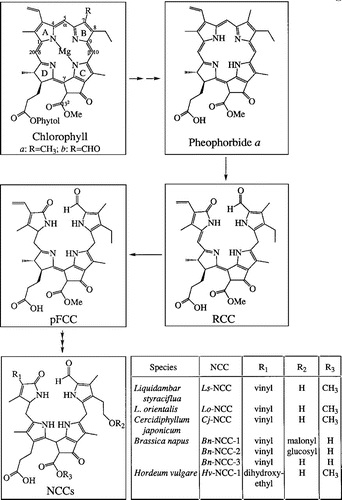
\includegraphics{figura1}
	\caption{Structuresofintermediary andfinalChlcatabolites arrangedaccordingtothe“pheophor-bide a oxygenase” (PaO) pathway of chlorophyll degradation. \cite{Matile1999}}
	\label{fig2}
\end{figure*}

\begin{figure*}[htb]
	\centering
	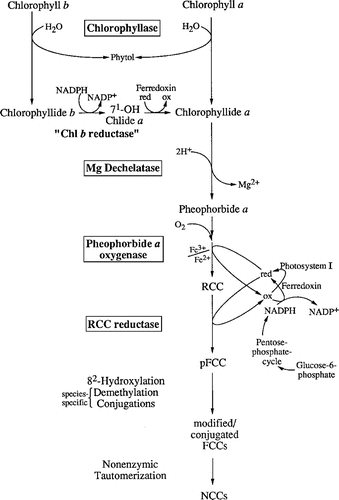
\includegraphics{figura2}
	\caption{The “pheophorbide a (PaO) pathway” of chlorophyll degradation in senescent leaves \cite{Matile1999}}
	\label{fig3}
\end{figure*}




\end{document}